\lhead{\emph{Implementation}}
\chapter{Implementation}
This chapter describes the different components of the Spatial Music Menu system. The main components includes a headset interface and an iOS application controlling the headset.

\section{Headset}
The headset interface used in this project is the Intelligent Headset (IHS)\footnote{\url{https://intelligentheadset.com/}}. The headset uses HRTF technology and can deliver spatial audio. 4 sensors are built into the headset; GPS, compass, gyroscope and accelerometer - making it possible to track head rotation and location of the user wearing it. The headset also includes 2 buttons - one in the outer center on each speaker. Connection to the headset is accessible via Bluetooth or wire. The headset is shown in figure?

[TODO: image of headset including button (2 images)]

The headset features can be exploited through mobile applications using an included SDK targeting the iOS and Android platform (iOS SDK currently at version 1.82 and an Android SDK running verson 1.21 \footnote{Version information from 05-05-2014. Developer site: \url{https://developer.intelligentheadset.com/our-sdk/}}). The platform used in this project is Apples iOS. The main reason for using this platform is that when this project started the Intelligent Headset only provided an SDK compatible with iOS and still - though accessible for the Android platform today - the iOS SDK is running a higher version number making it more mature i.e. stable.

The SDK is implemented in the Spatial Music Menu application. The Intelligent Headset API (Application Programming Interface) provides features like reading the raw sensor data from all sensors, button events and functions for headset connectivity and 3D audio handling. An overview of the components and their communication is shown in figure \ref{fig:implementationoverview}.

\begin{figure}[htbp]
	\centering
		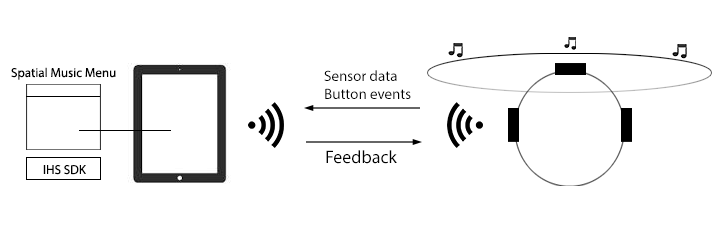
\includegraphics[width=\textwidth,height=\textheight,keepaspectratio]{./Figures/implementation_overview.png}
		\rule{35em}{1pt}
	\caption[Implementation overview]{An overview of the components of the implementation and their communication}
	\label{fig:implementationoverview}
\end{figure}


\section{Music}
We used Deezer\footnote{\url{https://www.deezer.com/}} as a music provider in the implementation. Deezer is a music streaming service and provides an iOS SDK for accessing different kinds of information through their API e.g. track info, user playlists, albums, streaming urls, etc.

The primary reason for choosing Deezer was that they provide previews of all music tracks (30 second clip). This is very convinient as it is not possible to spatialise audio streams using the IHS SDK. Instead the IHS SDK is quite limited in that the only way to place sound sources in the spatial audio space is to use 16-bit wav format. Deezers preview tracks comes in MP3 format so every track needed conversion to 16-bit wav before use. Download and conversion of music tracks was handled dynamically inside the Spatial Music Menu iOS application making it easier to add, remove and switch tracks. Basically one could add music tracks to the application by creating a Deezer playlist which is then synchronized by the iOS application. A synchronization operation is simply: 1) Getting the preview tracks MP3 url; 2) download all MP3 tracks and save on device; 3) convert all tracks to 16-bit wav and save on device. Besides preview audio the synchronization also included basic track information e.g. artist name, track name and album.


\section{Head Gestures Recognition}

DTW - Dynamic Time Warping 

Dynamic Time Warping \cite{salvador_toward_2007}

Accelerometer-based DTW \cite{akl_accelerometer-based_2010}

Start and end noise removal

Gyroscope + accelerometer data, 1 observation, 1 sequence


\section{iOS Application}
...
The iOS is a mature OS currently at version 7.1. The Spatial Music Menu are running version 6+ and optimized for the iPad.

As an overview and introduction of the iOS framework is out of this thesis scope - the interested reader is referred to Apples developer portal\footnote{\url{https://developer.apple.com/}} where a comprehensive documentation on the framework is available. Instead this section will focus on the application architecture, the design patterns and most important functionality of the Spatial Music Menu.

... following Apples best practice iOS design patterns\footnote{\url{https://developer.apple.com/library/ios/referencelibrary/GettingStarted/RoadMapiOS/DesignPatterns.html}}

\subsection{Overview}
An overview of the application architecture is shown in figure \ref{fig:apparchitecture}.

\begin{figure}[htbp]
	\centering
		\includegraphics[width=\textwidth,height=\textheight,keepaspectratio]{./Figures/app-architecture.pdf}
		\rule{35em}{1pt}
	\caption[App architecture]{iOS app architecture overview}
	\label{fig:apparchitecture}
\end{figure}

TODO: describe the architecture

- Singleton approach, iOS MVC pattern

\subsection{Settings views}
- TODO: show screenshots of iPad 3 views








